%============================================================================%
%
%	DOCUMENT DEFINITION
%
%============================================================================%

%we use article class because we want to fully customize the page and don't use a cv template
\documentclass[10pt,A4]{article}

%for commenting multiple lines out
\usepackage{verbatim}

%----------------------------------------------------------------------------------------
%	ENCODING
%----------------------------------------------------------------------------------------

% we use utf8 since we want to build from any machine
\usepackage[utf8]{inputenc}

%----------------------------------------------------------------------------------------
%	LOGIC
%----------------------------------------------------------------------------------------

% provides \isempty test
\usepackage{xstring, xifthen}

%----------------------------------------------------------------------------------------
%	FONT BASICS
%----------------------------------------------------------------------------------------

% some tex-live fonts - choose your own

%\usepackage[defaultsans]{droidsans}
%\usepackage[default]{comfortaa}
%\usepackage{cmbright}
\usepackage[default]{raleway}
%\usepackage{fetamont}
%\usepackage[default]{gillius}
%\usepackage[light,math]{iwona}
%\usepackage[thin]{roboto} 

% set font default
\renewcommand*\familydefault{\sfdefault}
\usepackage[T1]{fontenc}

% more font size definitions
\usepackage{moresize}

%----------------------------------------------------------------------------------------
%	FONT AWESOME ICONS
%---------------------------------------------------------------------------------------- 

% include the fontawesome icon set
\usepackage{fontawesome}

% use to vertically center content
% credits to: http://tex.stackexchange.com/questions/7219/how-to-vertically-center-two-images-next-to-each-other
\newcommand{\vcenteredinclude}[1]{\begingroup
\setbox0=\hbox{\includegraphics{#1}}%
\parbox{\wd0}{\box0}\endgroup}

% use to vertically center content
% credits to: http://tex.stackexchange.com/questions/7219/how-to-vertically-center-two-images-next-to-each-other
\newcommand*{\vcenteredhbox}[1]{\begingroup
\setbox0=\hbox{#1}\parbox{\wd0}{\box0}\endgroup}

% icon shortcut
\newcommand{\icon}[3] {
	\makebox(#2, #2){\textcolor{maincol}{\csname fa#1\endcsname}}
}

% icon with text shortcut
\newcommand{\icontext}[4]{
	\vcenteredhbox{\icon{#1}{#2}{#3}}  \hspace{2pt}  \parbox{0.9\mpwidth}{\textcolor{#4}{#3}}
}

% icon with website url
\newcommand{\iconhref}[5]{
    \vcenteredhbox{\icon{#1}{#2}{#5}}  \hspace{2pt} \href{#4}{\textcolor{#5}{#3}}
}

% icon with email link
\newcommand{\iconemail}[5]{
    \vcenteredhbox{\icon{#1}{#2}{#5}}  \hspace{2pt} \href{mailto:#4}{\textcolor{#5}{#3}}
}

%----------------------------------------------------------------------------------------
%	PAGE LAYOUT  DEFINITIONS
%----------------------------------------------------------------------------------------

% page outer frames (debug-only)
% \usepackage{showframe}		

% we use paracol to display breakable two columns
\usepackage{paracol}

% define page styles using geometry
\usepackage[a4paper]{geometry}

% remove all possible margins
\geometry{top=1cm, bottom=1cm, left=1cm, right=1cm}

\usepackage{fancyhdr}
\pagestyle{empty}

% space between header and content
% \setlength{\headheight}{0pt}

% indentation is zero
\setlength{\parindent}{0mm}

%----------------------------------------------------------------------------------------
%	TABLE /ARRAY DEFINITIONS
%---------------------------------------------------------------------------------------- 

% extended aligning of tabular cells
\usepackage{array}

% custom column right-align with fixed width
% use like p{size} but via x{size}
\newcolumntype{x}[1]{%
>{\raggedleft\hspace{0pt}}p{#1}}%


%----------------------------------------------------------------------------------------
%	GRAPHICS DEFINITIONS
%---------------------------------------------------------------------------------------- 

%for header image
\usepackage{graphicx}

% use this for floating figures
% \usepackage{wrapfig}
% \usepackage{float}
% \floatstyle{boxed} 
% \restylefloat{figure}

%for drawing graphics		
\usepackage{tikz}
\usetikzlibrary{shapes, backgrounds,mindmap, trees}

%----------------------------------------------------------------------------------------
%	Color DEFINITIONS
%---------------------------------------------------------------------------------------- 
\usepackage{transparent}
\usepackage{color}

% primary color
\definecolor{maincol}{RGB}{ 225, 0, 0 }

% accent color, secondary
% \definecolor{accentcol}{RGB}{ 250, 150, 10 }

% dark color
\definecolor{darkcol}{RGB}{ 70, 70, 70 }

% light color
\definecolor{lightcol}{RGB}{245,245,245}


% Package for links, must be the last package used
\usepackage[hidelinks]{hyperref}

% returns minipage width minus two times \fboxsep
% to keep padding included in width calculations
% can also be used for other boxes / environments
\newcommand{\mpwidth}{\linewidth-\fboxsep-\fboxsep}



%============================================================================%
%
%	CV COMMANDS
%
%============================================================================%

%----------------------------------------------------------------------------------------
%	 CV LIST
%----------------------------------------------------------------------------------------

% renders a standard latex list but abstracts away the environment definition (begin/end)
\newcommand{\cvlist}[1] {
	\begin{itemize}{#1}\end{itemize}
}

%----------------------------------------------------------------------------------------
%	 CV TEXT
%----------------------------------------------------------------------------------------

% base class to wrap any text based stuff here. Renders like a paragraph.
% Allows complex commands to be passed, too.
% param 1: *any
\newcommand{\cvtext}[1] {
	\begin{tabular*}{1\mpwidth}{p{0.98\mpwidth}}
		\parbox{1\mpwidth}{#1}
	\end{tabular*}
}

%----------------------------------------------------------------------------------------
%	CV RIGHT SECTION
%----------------------------------------------------------------------------------------

% Renders a a CV section headline with a nice underline in main color.
% param 1: section title
\newcommand{\cvsection}[1] {
	\vspace{10pt}
	\cvtext{
		\textbf{\LARGE{\textcolor{darkcol}{\uppercase{#1}}}}\\[-6pt]
		\textcolor{maincol}{ \rule{0.1\textwidth}{2pt} } \\
	}
	\vspace{0pt}
}

%----------------------------------------------------------------------------------------
%	CV LEFT SECTION
%----------------------------------------------------------------------------------------

% Renders a a CV section headline with a nice underline in main color.
% param 1: section title
\newcommand{\cvleftsection}[1] {
	\vspace{9pt}
	\cvtext{
		\textbf{\large{\textcolor{darkcol}{\uppercase{#1}}}}\\[-6pt]
		\textcolor{maincol}{ \rule{0.1\textwidth}{2pt} } \\
	}
	\vspace{-3pt}
}

%----------------------------------------------------------------------------------------
%	META SKILL
%----------------------------------------------------------------------------------------

% Renders a progress-bar to indicate a certain skill in percent.
% param 1: name of the skill / tech / etc.
% param 2: level (for example in years)
% param 3: percent, values range from 0 to 1
\newcommand{\cvskill}[3] {
	\begin{tabular*}{1\mpwidth}{p{0.72\mpwidth}  r}
 		\textcolor{black}{\textbf{#1}} & \textcolor{maincol}{#2}\\
	\end{tabular*}%

	\hspace{0pt}
	\begin{tikzpicture}[scale=1,rounded corners=2pt,very thin]
		\fill [lightcol] (0,0) rectangle (1\mpwidth, 0.15);
		\fill [maincol] (0,0) rectangle (#3\mpwidth, 0.15);
  	\end{tikzpicture}%
}

%----------------------------------------------------------------------------------------
%	META SKILL
%----------------------------------------------------------------------------------------

% Renders a progress-bar to indicate a certain skill in percent.
% param 1: name of the skill / tech / etc.
% param 2: level (for example in years)
\newcommand{\cvother}[2] {
	\begin{tabular*}{1\mpwidth}{p{0.72\mpwidth}  r}
 		\textcolor{black}{\textbf{#1}} & \textcolor{maincol}{#2}\\
	\end{tabular*}%


}


%----------------------------------------------------------------------------------------
%	 CV EVENT
%----------------------------------------------------------------------------------------

% Renders a table and a paragraph (cvtext) wrapped in a parbox (to ensure minimum content
% is glued together when a pagebreak appears).
% Additional Information can be passed in text or list form (or other environments).
% the work you did
% param 1: time-frame i.e. Sep 14 - Jan 15 etc.
% param 2:	 event name (job position etc.)
% param 3: Customer, Employer, Industry
% param 4: Short description
% param 5: work done (optional)
% param 6: technologies include (optional)
% param 7: achievements (optional)
\newcommand{\cvevent}[7] {

	% we wrap this part in a parbox, so title and description are not separated on a pagebreak
	% if you need more control on page breaks, remove the parbox
	\parbox{\mpwidth}{
		\begin{tabular*}{1\mpwidth}{p{0.6\mpwidth}  r}
	 		\textcolor{black}{\textbf{#2}} & \colorbox{maincol}{\makebox[0.35\mpwidth]{\textcolor{white}{#1}}} \\
			\textcolor{maincol}{\textbf{#3}} & \\
		\end{tabular*}\\[5pt]

		\ifthenelse{\isempty{#4}}{}{
			\cvtext{#4}\\
		}
	}

	\ifthenelse{\isempty{#5}}{}{
		\vspace{0pt}
		{#5}
	}

	\ifthenelse{\isempty{#6}}{}{
		\vspace{5pt}
		\cvtext{\textbf{Technology Stack:}}\\[-7pt]
		\vspace{-3mm}
		{#6}
	}

	\ifthenelse{\isempty{#7}}{}{
		% \vspace{5pt}
		\cvtext{\textbf{Achievements:}}\\[-7pt]
		{#7}
	}
	\vspace{15pt}
}

%----------------------------------------------------------------------------------------
%	 CV EVENT
%----------------------------------------------------------------------------------------

% Renders a table and a paragraph (cvtext) wrapped in a parbox (to ensure minimum content
% is glued together when a pagebreak appears).
% Additional Information can be passed in text or list form (or other environments).
% the work you did
% param 1: time-frame i.e. Sep 14 - Jan 15 etc.
% param 2:	 event name (job position etc.)
% param 3: Customer, Employer, Industry
% param 4: Short description
% param 5: work done (optional)
% param 6: technologies include (optional)
% param 7: achievements (optional)
\newcommand{\cvminievent}[3] {

	% we wrap this part in a parbox, so title and description are not separated on a pagebreak
	% if you need more control on page breaks, remove the parbox
	\parbox{\mpwidth}{
		\begin{tabular*}{1\mpwidth}{p{0.55\mpwidth}  r}
	 		\textcolor{black}{\textbf{#2}} & \colorbox{maincol}{\makebox[0.4\mpwidth]{\textcolor{white}{#1}}} \\
			\textcolor{maincol}{\textbf{#3}} & \\
		\end{tabular*}

	}

}



%----------------------------------------------------------------------------------------
%	 CV META EVENT
%----------------------------------------------------------------------------------------

% Renders a CV event on the sidebar
% param 1: title
% param 2: subtitle (optional)
% param 3: customer, employer, etc,. (optional)
% param 4: info text (optional)
\newcommand{\cvmetaevent}[4] {
    \vspace{-7pt}
	\textcolor{maincol} {\cvtext{\textbf{\begin{flushleft}#1\end{flushleft}}}}\\[-5pt]

	\ifthenelse{\isempty{#2}}{}{
	\textcolor{darkcol} {\cvtext{\textbf{#2}} }
	}

	\ifthenelse{\isempty{#3}}{}{
		\cvtext{{ \textcolor{darkcol} {#3} }}\\
	}

	\cvtext{#4}\\[-25pt]
	\vspace{27pt}
}

%---------------------------------------------------------------------------------------
%	QR CODE
%----------------------------------------------------------------------------------------

% Renders a qrcode image (centered, relative to the parentwidth)
% param 1: percent width, from 0 to 1
\newcommand{\cvqrcode}[1] {
	\begin{center}
		
\includegraphics[width={#1}\mpwidth]{images/linkedinQR.png}
	\end{center}
}


%============================================================================%
%
%
%
%	DOCUMENT CONTENT
%
%
%
%============================================================================%
\begin{document}
\columnratio{0.31}
\setlength{\columnsep}{2.2em}
\setlength{\columnseprule}{4pt}
\colseprulecolor{lightcol}
\begin{paracol}{2}
\begin{leftcolumn}
%---------------------------------------------------------------------------------------
%	META IMAGE
%----------------------------------------------------------------------------------------
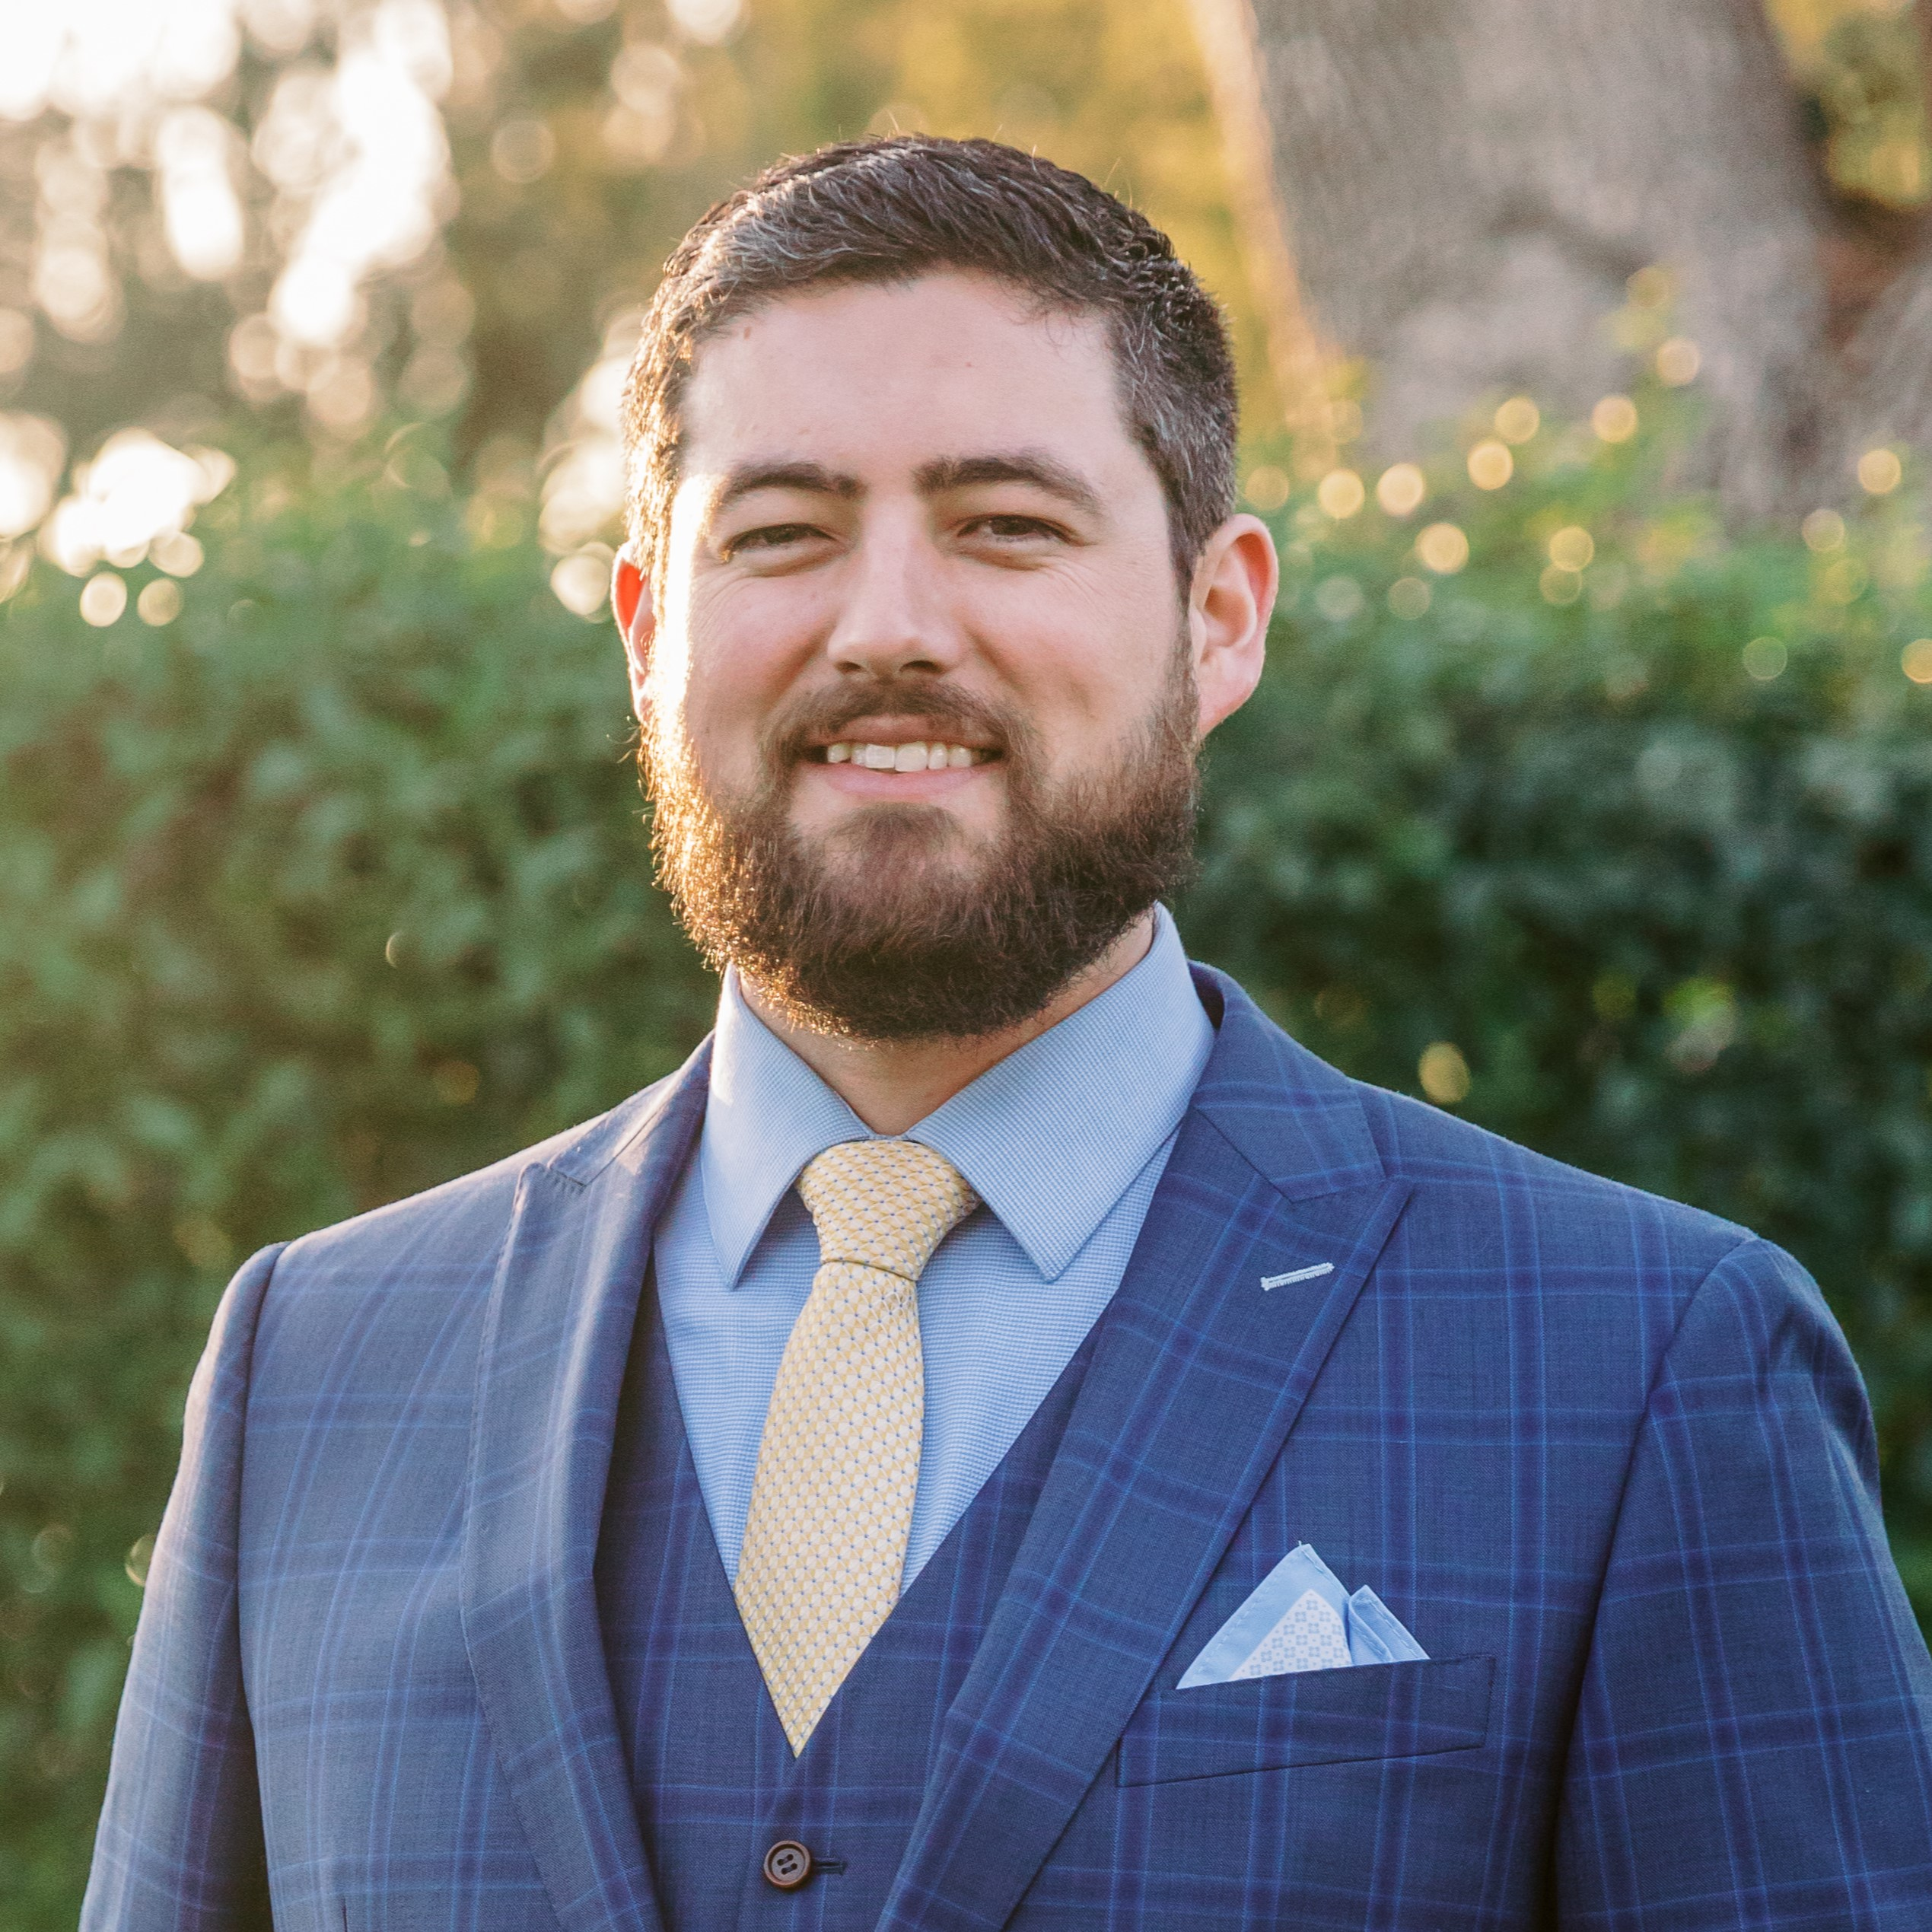
\includegraphics[width=\linewidth]{images/headshot.jpg}	%trimming relative to image size

%---------------------------------------------------------------------------------------
%	META SKILLS
%----------------------------------------------------------------------------------------
\cvleftsection{Languages}

\cvother{Java 13+} {5 yrs} \\[-2pt] %{1}

\cvother{SQL} {5 yrs} \\[-2pt] %{.75}

\cvother{Javascript/Typescript} {9 mo} \\[-2pt] %{.75}

\cvother{Python} {1+ yrs}  \\[-2pt] %{.5}

\begin{comment}
\cvleftsection{TECHNOLOGIES}

\cvother{Spring Boot} {5 yrs} \\[-2pt]

\cvother{Gradle} {5 yrs}  \\[-2pt] %{1}

\cvother{Kafka} {3 yrs} \\[-2pt]

\cvother{RabbitMQ} {3 yrs} \\[-2pt]

\cvother{React} {9 mo} \\[-2pt]

\end{comment}

\cvleftsection {TOOLS}

\cvother{Intellij} {3 yrs} \\[-2pt]

\cvother{VsCode} {2 yrs} \\[-2pt]

\cvother{NeoVim} {3+ yrs} \\[-2pt]

\cvother{Atlassian Suite} {5 yrs} \\[-2pt]


\begin{comment}
%\vfill\null
\cvleftsection{CONTACT}

\icontext{MapMarker}{12}{3708 Windstone Dr.\\Plano TX, 75023}{black}\\[6pt]
\icontext{MobilePhone}{12}{+1 916 801 6154}{black}\\[6pt]
\iconemail{Envelope}{12}{casada94@gmail.com}{casada94@gmail.com}{black}\\[6pt]
\end{comment}
%\vfill\null
%\cvqrcode{0.7}

%---------------------------------------------------------------------------------------
%	EDUCATION
%----------------------------------------------------------------------------------------
%\newpage
\cvleftsection{EDUCATION}

\cvmetaevent
{08/15/2022 - 05/15/2024}
{M.S. Computer Science}
{C.S.U., Long Beach \hfill \textcolor{maincol}{\textbf{GPA: 4.0}}}
{Computer Science Master’s Program with thesis on AI/ML.  I graduated 2nd in my class and introduced a novel dropout out technique in my thesis, ’Sector-Wise Dropout’.}

\cvmetaevent
{08/15/2015 - 05/15/2020}
{B.S. Computer Science.}
{C.S.U., Long Beach}
{}

\vfill\null
\cvqrcode{0.6}

%---------------------------------------------------------------------------------------
%	CERTIFICATION
%----------------------------------------------------------------------------------------
%\newpage
\begin{comment}
\cvleftsection{CERTIFICATIONS}

\cvmetaevent
{Online Classes}
{}
{}
{It is important for me to continuously learn and grow my capabilities. Therefore, I keep myself up to date with online classes through TCS and have enrolled in a Masters Program as California State University, Long Beach.}

%\vfill
%\cvqrcode{0.7}

%\newpage
%\mbox{} % hotfix to place qrcode on the bottom when there are not other elements
%\vfill
%\cvqrcode{0.7}
\end{comment}
\end{leftcolumn}
\begin{rightcolumn}
%---------------------------------------------------------------------------------------
%	TITLE  HEADER
%----------------------------------------------------------------------------------------
\fcolorbox{white}{darkcol}{\begin{minipage}[c][3.5cm][c]{1\mpwidth}
	\begin {center}
		\HUGE{ \textbf{ \textcolor{white}{ \uppercase{ Clayton Asada } } } } \\[-24pt]
		\textcolor{white}{ \rule{0.3\textwidth}{1.25pt} } \\[8pt]
		%\large{ \textcolor{white} {Software Engineer} } \\[4pt]
		\large{\textcolor{white} { Plano, TX ---}}
		\large{\textcolor{white} { (916) 801 6154 ---}}
		\large{\textcolor{white} { Casada94@gmail.com   } }
	\end {center}
\end{minipage}} \\[14pt]
\vspace{-12pt}

%---------------------------------------------------------------------------------------
%	PROFILE
%----------------------------------------------------------------------------------------
%\vfill\null
\cvsection{PROFILE}

\cvtext{I'm a highly motivated, results-driven software engineer with a stong background in Java development, cloud technologies, and AI/ML. I thrive in dynamic environments, consistently delivering innovative solutions that enhance system performance and drive business growth. My expertise spans across designing and maintaining applications, integrating APIs, and implementing cutting-edge technologies to meet evolving business needs. I am passionate about leveraging my skills to positively impact projects and continuously expand my knowledge in the ever-evolving tech landscape.
}

%---------------------------------------------------------------------------------------
%	WORK EXPERIENCE
%----------------------------------------------------------------------------------------
%\vfill\null
\cvsection{WORK EXPERIENCE}

\cvevent
	{07/15/2024 - 05/05/2025}
	{Senior Software Engineer}
  {Raytheon}
	{Modernize, enhance, and maintain both backend and frontend codebases. Incorporating new technologies and libraries to deliver new features and/or improve readability, testability, and maintainability.}
	{\cvlist{
		\item Frontend: develop common React.js components for multiple user-facing products
		\item Backend: Update and enhance Spring Boot microservices for large data processing and API’s for powering client focused products	
	}}
	{
	\begin{table}[h!]
		\begin{tabular}{p{2.5cm} p{2.5cm} p{2.5cm} p{2.5cm} p{2.5cm} }
			
\includegraphics[width=.5cm, height=.5cm]{icons/icons8-spring-boot-120.png} Spring Boot		& 
\includegraphics[width=.5cm, height=.5cm]{icons/icons8-react-96.png} React		& 
\includegraphics[width=.5cm, height=.5cm]{icons/icons8-amazon-web-services-120.png} AWS		& 
\includegraphics[width=.5cm, height=.5cm]{icons/icons8-mysql-logo-120.png} MySql		& 
\includegraphics[width=.5cm, height=.5cm]{icons/icons8-linux-96.png} Linux		\\
    	\end{tabular}
	\end{table}
	}
	{\cvlist{
		\item Guided by user feedback, I created a feature to help users quickly identify the topics and context of their next task, which improved their efficiency and task throughput.	
	}}
\cvevent
	{07/15/2024 - 05/05/2025}
	{Software Engineer}
  {U.S. Department of Defense}
	{Modernize, enhance, and maintain both backend and frontend codebases. Incorporating new technologies and libraries to deliver new features and/or improve readability, testability, and maintainability.}
	{\cvlist{
		\item Frontend: develop common React.js components for multiple user-facing products
		\item Backend: Update and enhance Spring Boot microservices for large data processing and API’s for powering client focused products	
	}}
	{
	\begin{table}[h!]
		\begin{tabular}{p{2.5cm} p{2.5cm} p{2.5cm} p{2.5cm} p{2.5cm} }
			
\includegraphics[width=.5cm, height=.5cm]{icons/icons8-spring-boot-120.png} Spring Boot		& 
\includegraphics[width=.5cm, height=.5cm]{icons/icons8-react-96.png} React		& 
\includegraphics[width=.5cm, height=.5cm]{icons/icons8-amazon-web-services-120.png} AWS		& 
\includegraphics[width=.5cm, height=.5cm]{icons/icons8-mysql-logo-120.png} MySql		& 
\includegraphics[width=.5cm, height=.5cm]{icons/icons8-linux-96.png} Linux		\\
    	\end{tabular}
	\end{table}
	}
	{\cvlist{
		\item Guided by user feedback, I created a feature to help users quickly identify the topics and context of their next task, which improved their efficiency and task throughput.	
	}}

\cvevent
	{03/15/2021 - 07/15/2024}
	{Java Developer}
	{Tata Consultancy Services: Experian}
	{Drive progress in a company-wide modernization and migration project.  Design, develop, and maintain new applications, including database tables, for AWS cloud deployment}
	{
	\begin{table}[h!]
		\begin{tabular}{p{2.5cm} p{2.5cm} p{2.5cm} p{2.5cm} p{2.5cm} }
			
\includegraphics[width=.5cm, height=.5cm]{icons/icons8-spring-boot-120.png} Spring Boot		& 
\includegraphics[width=.5cm, height=.5cm]{icons/icons8-amazon-web-services-120.png} AWS		& \includegraphics[width=.5cm, height=.5cm]{icons/apache-kafka_icon_138937.png} Kafka		& 
\includegraphics[width=.5cm, height=.5cm]{icons/icons8-mysql-logo-120.png} MySql		& 
\includegraphics[width=.5cm, height=.5cm]{icons/icons8-jenkins-120.png} Jenkins		\\
    	\end{tabular}
	\end{table}
	}
	{\cvlist{
		\item My Hackathon idea, inspired by customer conversions, lead to implementation, completed by me, which increased yearly revenue by ~\$800,000 (16\%)
		\item Performance improvements of two legacy applications, resulting in 50\% reduction in latency
	}}

\cvminievent
{07/-1/2012 - 09/01/2015}
{Electrical Systems Technician}
{United State Marine Corps}



% hotfixes to create fake-space to ensure the whole height is used
% \mbox{}
% \vfill
\mbox{}
\vfill
\mbox{}
\vfill
\mbox{}
\end{rightcolumn}
\end{paracol}
\end{document}
